\documentclass{ctexart}
\usepackage{PhysicalChemistryNote}

\begin{document}\pagestyle{plain}
\noindent\tbf{\LARGE 1C 实际气体}\vspace{15pt}\\
\indent “有时,你会发现科学家们做的假设也许比你的新年计划还要理想”.\\
\indent 实验发现,在实际情况下,真实气体的行为与理想气体状态方程有明显偏差.%
造成这一偏差是由于低温高压时,气体分子之间间距减小,其本身的体积不能再忽略不计,也不能看作弹性质点,%
\tbf{1B.1.1}的假设就失效了.%
基于此,人们提出了对理想气体状态方程的修正,即各类实际气体的状态方程.%
\vspace{12pt}\\
\Section{1C.1 实际气体的行为}
\Part{压缩因子与波义耳温度}
\indent 实际气体,由于我们在本节导言中提到的原因,以及分子间作用力的缘故,常常会与理想气体状态方程有所偏离.%
我们需要定义一个能描述这种偏离的大小的参数.
\begin{definition}[1C.1.1 实际气体的压缩因子]
    定义压缩因子
    \[Z=\dfrac{p\Vm}{RT}=\dfrac{pV}{nRT}\]
    以衡量实际气体与理想气体的偏差程度.
\end{definition}
压缩因子实际上反映了受到同样压力时,实际气体与理想气体的摩尔体积之比.%
因此,压缩因子$Z$越大,实际气体越难被压缩(即难以液化).%
可以预见的是,当压力$p\to0$时,所有气体都符合理想气体状态方程,因此此时$Z\to1$.\\
\indent 一般来说,实际气体的$Z-p$曲线有两种类型.一种是随着$p$增大而单调增大,一种是随着$p$增大先减小后增大,如下图所示.\\
\begin{figure}[h]
    \centering\documentclass{standalone}
\usepackage{PhysicalChemistryNote}
\begin{document}
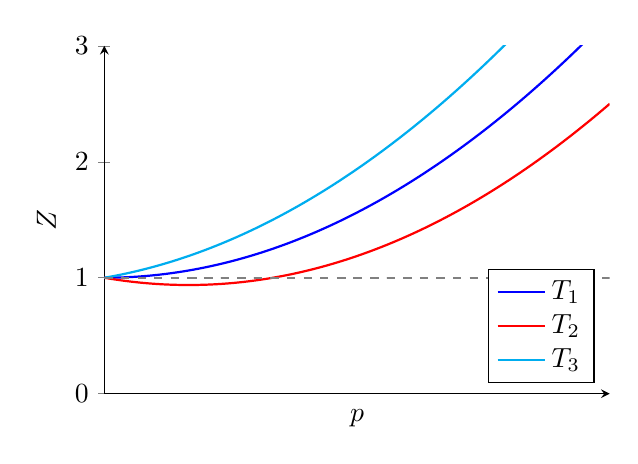
\begin{tikzpicture}
    \begin{axis}[
        width = 8cm,
        height = 6cm,
        legend pos = south east,
        xlabel = {$p$},
        ylabel = {$Z$},
        axis lines = left,
        ymin = 0,
        ymax = 3,
        xtick = \empty,
        domain = 0:3,
        samples = 400
    ]
    \addplot [thick, blue] {0.25*x^2+1};
    \addplot [thick, red] {0.25*(x-0.5)^2+15/16};
    \addplot [thick, cyan] {0.25*(x+0.5)^2+15/16};
    \addplot [thick, dashed, gray] {1};
    \legend {$T_1$,$T_2$,$T_3$}
    \end{axis}
\end{tikzpicture}
\end{document}
\end{figure}\\
\indent 在某个特定的温度(即图中的$T_1$)下,当压力在$p=0$附近的一定范围内,$Z$的变化都不大,即满足
\[\left(\dfrac{\p Z}{\p p}\right)_{T,p\to0}=0\]
时,在这一范围内用理想气体状态方程描述实际气体的偏差都是十分小的.%
这时的$Z-p$曲线满足$p=0$时$Z$对$p$的偏导数为$0$.对这样的温度$T_1$,我们做如下定义.
\begin{definition}[1C.1.2 实际气体的波义耳温度]
    定义实际气体的\tbf{波义耳温度}$T_B$为使得
    \[\left(\dfrac{\p\left(p\Vm\right)}{\p p}\right)_{T_B,p\to0}=0\]
    的温度.
\end{definition}
当温度低于$T_B$时,$\left(\dfrac{\p\left(p\Vm\right)}{\p p}\right)_{T_B,p\to0}<0$.根据导数的知识,存在一段压强范围使得$Z<1$,即气体容易被压缩而液化.%
反之,当温度高于$T_B$时,恒有$Z>1$,气体难以被压缩而液化.%
\vspace{4pt}\\
\Part{实际气体的$p-V$图}
\indent 除了$Z-p$图之外,我们还有一种描述实际气体行为的图像,即定温条件下的$p-\Vm$图.我们给出$\text{CO}_2$在各个温度下的$p-\Vm$图以供参考(原谅笔者懒得自己画于是找了一张图).
\begin{figure}[H]
    \centering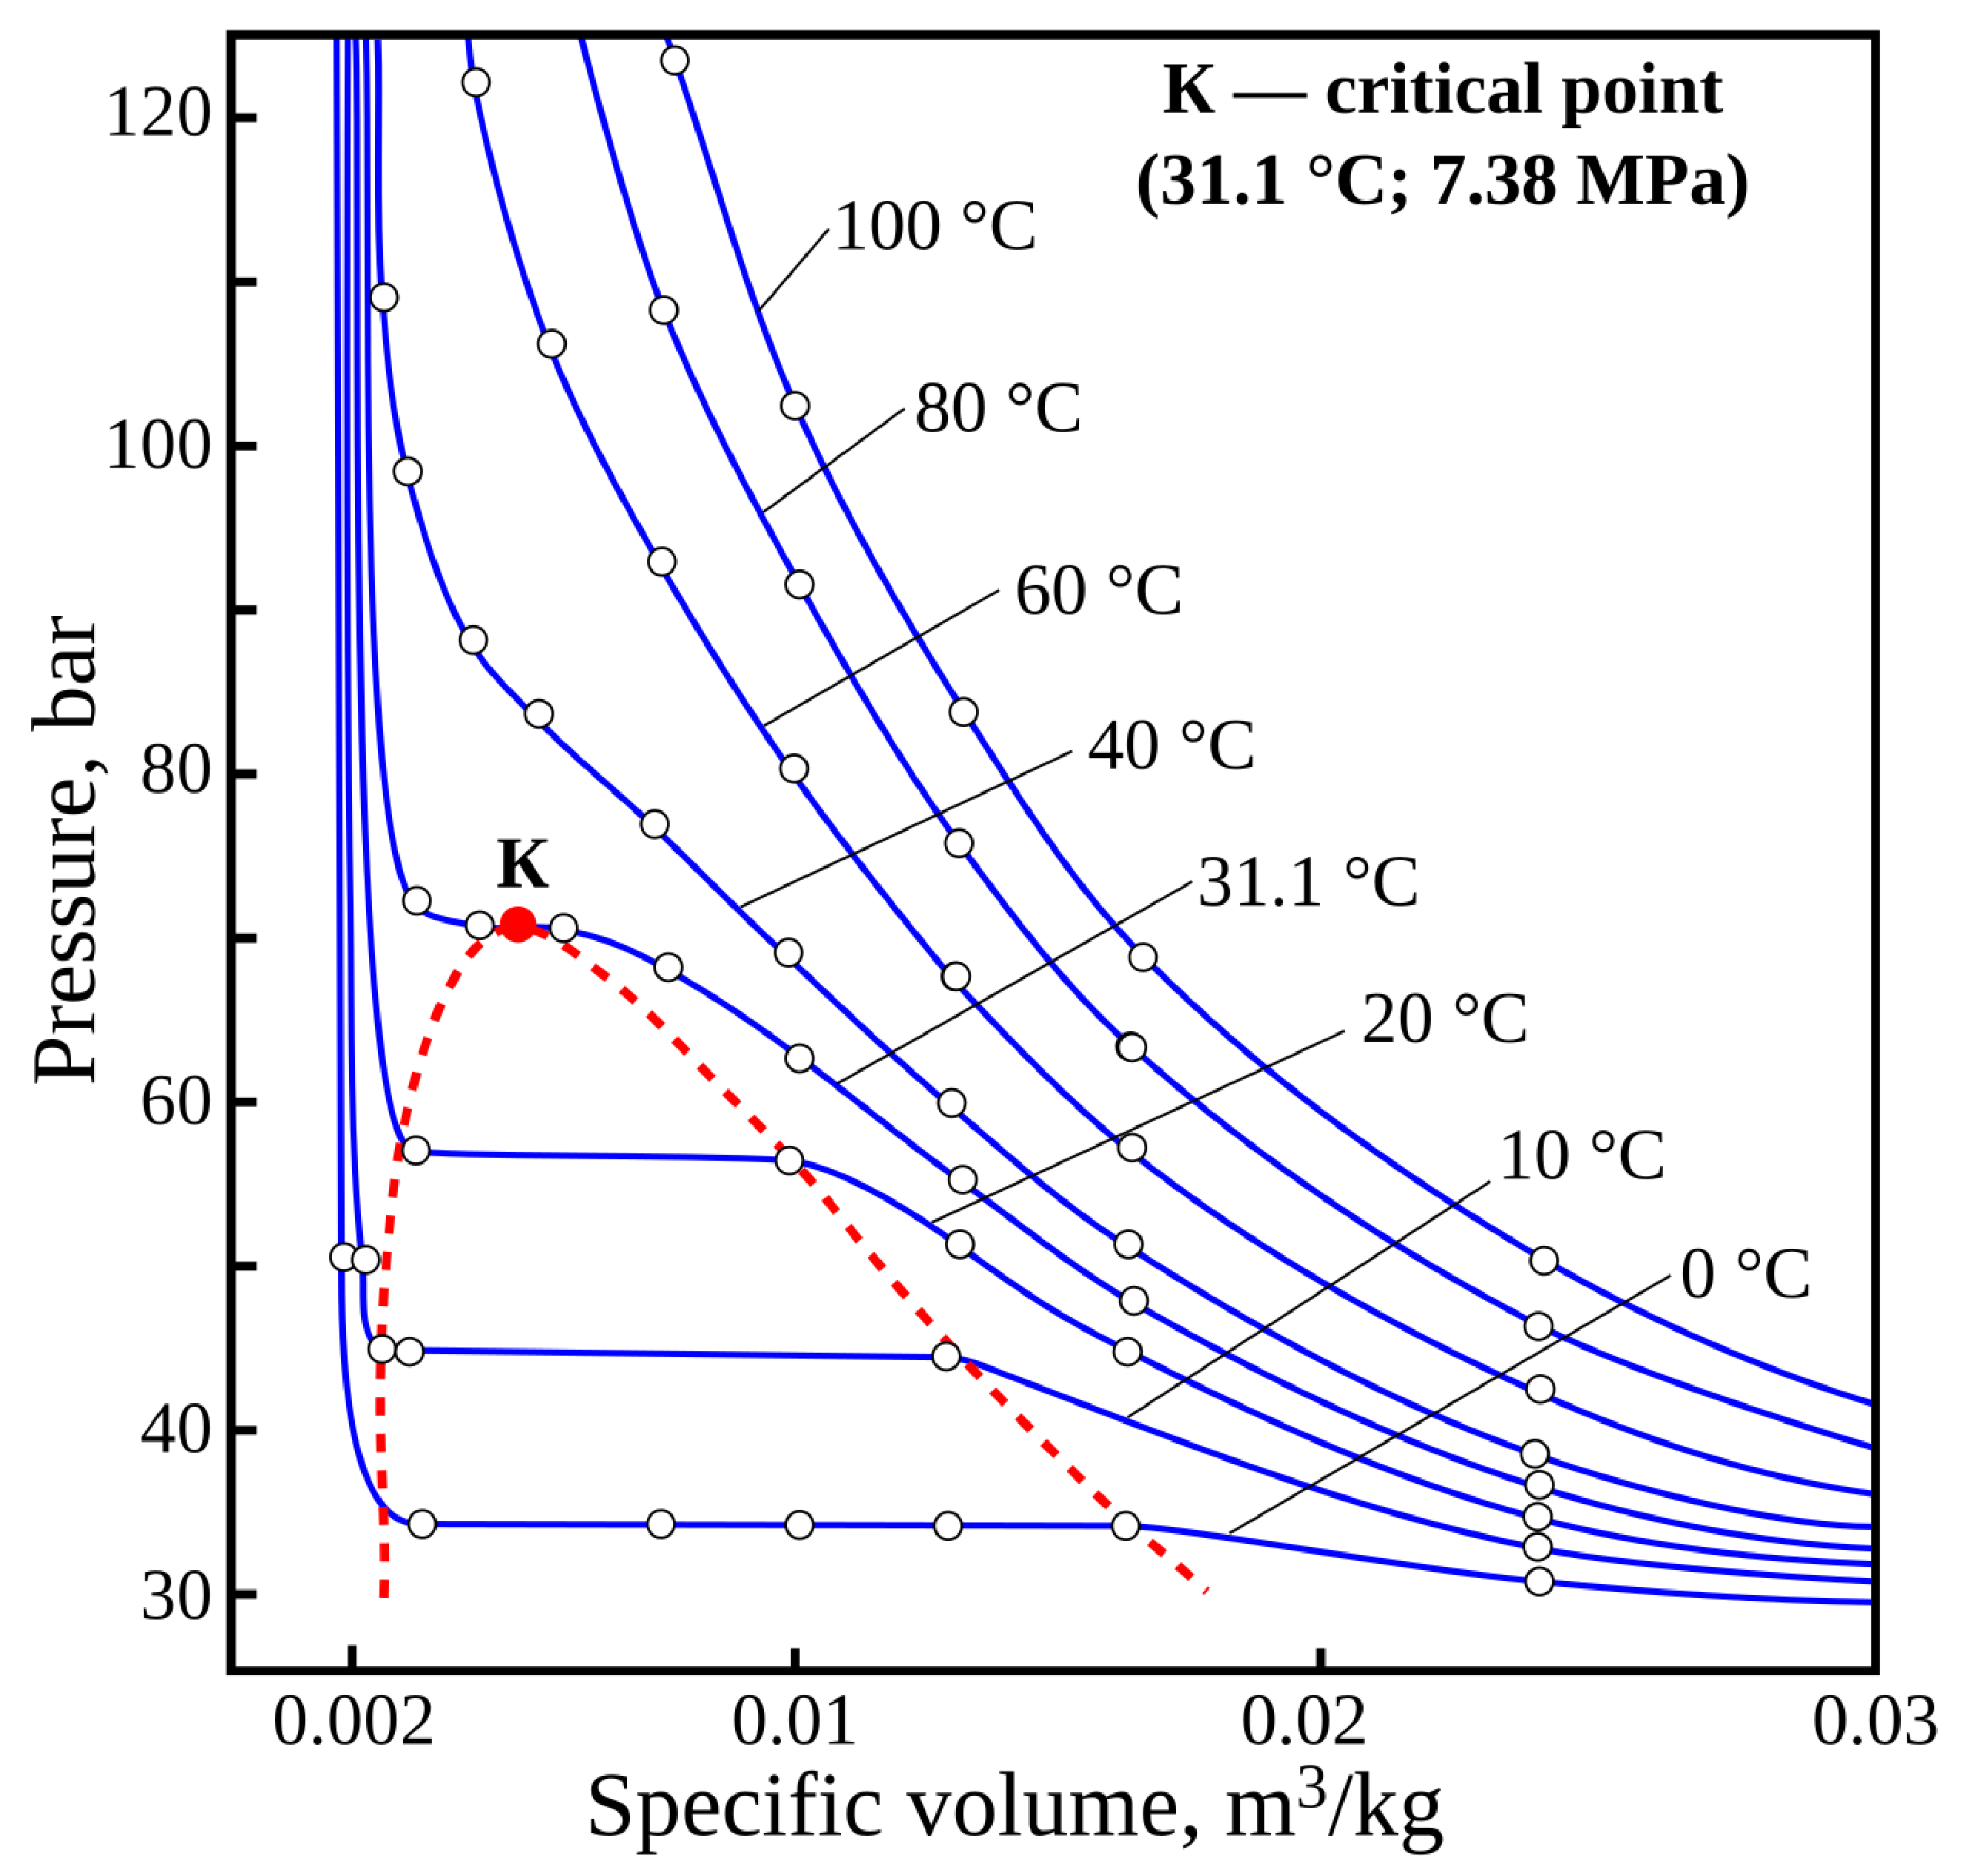
\includegraphics[scale=0.2]{picture/realCO2p-V.eps}
\end{figure}
上图中的曲线大致可以分为三类.\\
\indent 在较低的温度下,曲线大致可以分为三段.当$\Vm$较大时,曲线符合气体的一般性质,即体积减小(压缩)时压力增大.%
然而,中间出现了一段水平线,表明此时压缩并不改变体系的压力.由此可以想见,气体在此过程中发生了液化,这条线上$\Vm$的减小表示液相占比的增多.%
最后一段时,已经完全是液体,压力线陡然上升,表示液体不易压缩.\\
\indent 在较高的温度下,曲线大致符合等轴双曲线的形状,即$pV=C$,表示此时$\text{CO}_2$的性质与理想气体差别不大.\\
\indent 我们注意到在这些曲线中有这样特殊的一条:等温线的水平部分缩成一点,在此出现\tbf{拐点}.
\begin{hint}
    曲线的\tbf{拐点}的严格定义是曲线凹凸性发生改变的点.对于一个函数$f(x)$,如果点$\left(x_0,f\left(x_0\right)\right)$是此函数(图像)的拐点,那么我们有%
    $f'\left(x_0\right)=f''\left(x_0\right)=0\neq f'''\left(x_0\right)$.
\end{hint}
你可以注意到,在这条线上方,不再出现表示气液共存的水平线.这代表一个简单的事实:在此曲线对应的温度之上,你无论如何操作都不再能得到液体.%
反之,在此温度之下,总存在气液共存的状态.我们给这一特殊的温度及其状态做如下定义.
\begin{definition}[1C.1.3 临界态与超临界态]
    \tbf{临界态}是指纯物质的气,液两相平衡共存的极限状态.此时的温度为\tbf{临界温度}$T_\text c$,%
    此时的压力为\tbf{临界压力}$p_\text c$,体积为\tbf{临界体积}$V_\text c$,统称为\tbf{临界常数}.该状态对应的等温线为\tbf{临界等温线}.\\
    温度高于临界温度,压力高于临界压力的状态即为\tbf{超临界态}.
\end{definition}
在临界态下,气-液两相的一切差别都消失了,比体积相同,表面张力为零,汽化热为零,因而气液两相的界面也将消失.%
在超临界态下,物质兼具气体和液体的性质,在工业上也有一定的应用(例如用超临界$\text{CO}_2$萃取咖啡因).\\
\indent 我们对上述图中的区域也做一些描述.高于临界等温线的区域为单相区域,如果此时压力还高于临界压力,那么物质为超临界态,否则为气态;%
温度低于临界温度时,中间的帽形区域为气液两相共存的区域,帽形区域的边界与临界等温线所夹区域的左半部分为纯液相,右半部分为纯气相.\\
\indent 可以看出,当压力足够低或温度足够高时,气体总是无法液化,说明分子间作用力并不显著.此时的气体接近于理想气体.%
\vspace{12pt}\\
\Section{1C.2 维里(位力)方程}
\indent 对于现实中的问题,我们很难用纯理论化的方式对其进行量化.迄今以来,以及你以后看到的许多公式都只存在纸面上,尽管再精密,都和现实世界有一定的差距.%
实际气体的状态方程就是这样的问题.不过,我们还有一计:用足够多的参数拟合.\\
\indent 维里方程,又称为维里展开(virial expansion,此处的维里和位力都是音译),由Kammerlingh Onnes提出,就是这样的一个用于拟合实际气体状态方程的方法.
\begin{theorem}[1C.2 维里方程]
    在一定的温度下,压缩因子$Z$应当是$p$或者$\dfrac{1}{V_\text m}$的函数.\\
    将$Z$对$p$做级数展开,则有
    \[Z=1+B'p+C'p^2+\cdots\]
    或者更常见地,对$\dfrac{1}{V_\text m}$做级数展开
    \[Z=1+\dfrac{B}{\Vm}+\dfrac{C}{\Vm^2}+\cdots\]
    系数$B',C',\cdots$或$B,C,\cdots$被称为第二,第三,$\cdots$\tbf{维里系数},它们是关于温度的函数.\\
    维里系数可以通过测定实际气体的$p-\Vm-T$数据后拟合得到.
\end{theorem}
在这里,我们需要做一些额外的说明.我们所说的压力$p\to0$时,实际气体符合理想气体状态方程,\tbf{并非}符合理想气体的所有性质.%
例如,理想气体的压缩因子$Z$不论何时都等于$1$,因此对$p$的变化率$\dfrac{\di Z}{\di p}=0$.%
然而,对于符合维里方程(我们采取第一种形式)的实际气体,则有
\[\dfrac{\di Z}{\di p}=B'+2C'p+\cdots\]
当$p\to0$时有$\dfrac{\di Z}{\di p}=B'$.因此,变化率这一性质不一定与理想气体相符.%
然而,当上式中$B'=0$时,我们有
\[\left(\dfrac{\p\left(p\Vm\right)}{\p p}\right)_{T_B,p\to0}=\left(\dfrac{\di Z}{\di p}\right)_{p\to0}=B'=0\]
此时对应的温度即为波义耳温度.在波义耳温度下,气体符合$pV\approx nRT$的压力范围比其它温度下更宽.\\
\indent 维里方程在实际生产过程中应用广泛(只要你的数据测得够多够准,你就可以得到足够精度的方程),%
并且无需对底层的热力学有了解.它甚至还可以用于液体和固体的状态方程.所谓参数够多,你就是造物主.%
\vspace{12pt}\\
\Section{1C.3 van der Waals方程}
\Part{van der Waals方程及其物理意义}
\indent 在所有描述实际气体的状态方程中,van der Waals(范德华)方程是最有名的.不仅是因为它与实验数据符合的相当好,%
还因它对理想气体状态方程进行了有物理意义的修正,而非简单的拟合(比如那些费尽心思凑出符合实验数据的公式的可怜的科研人员们).%
\begin{theorem}[1C.3.1 van der Waals 方程]
    我们有
    \[\left(p+\dfrac{a}{\Vm^2}\right)\left(\Vm-b\right)=RT\]
    其中$a,b$为修正项,其物理意义将在接下来叙述.
\end{theorem}
\begin{derivation}
    我们来讨论如何得到这两个修正项.\\
    理想气体状态方程$p\Vm=RT$中的$\Vm$应当指气体分子能自由活动的体积.%
    现实世界中,我们不能忽略分子自身的体积,因此$\Vm$需要减去体积修正项$b$.\\
    我们仍然拿出我们的边长为$l$的正方体容器,并且向其中一个一个地加入半径为$r$的球体分子.\\
    计算这些气体分子能自由活动的范围时,我们仍然把它们抽象成质点,但是任意两个质点之间的间距不能小于$2r$.\\
    放入第一个分子$X_1$,它与所有壁都至少应保持$r$的距离(后面的分子也一样),因此它能自由活动的体积为
    \[V_{1,\text{free}}=\left(l-2r\right)^3\]
    第二个分子$X_2$除了与器壁保持不小于$r$的距离之外,还要求不能进入以第一个分子为球心,半径为$2r$的球内.因此$X_2$能自由活动的体积为
    \[V_{2,\text{free}}=\left(l-2r\right)^3-\dfrac43\pi\left(2r\right)^3\]
    依次类推,放入第$N$个分子$X_N$后,它能自由活动的体积为
    \[V_{N,\text{free}}=\left(l-2r\right)^3-(N-1)\cdot\dfrac43\pi\left(2r\right)^3\]
    平均来说,每个分子能自由活动的体积为
    \[\begin{aligned}
        \overline{V_{\text{free}}}
        &= \dfrac{1}{N}\sum_{i=1}^{N}V_{i,\text{free}} \\
        &= \dfrac{1}{N}\sum_{i=1}^{N}\left(\left(l-2r\right)^3-(i-1)\cdot\dfrac43\pi\left(2r\right)^3\right) \\
        &= (l-2r)^2-\dfrac1N\cdot\dfrac{N(N-1)}{2}\cdot\dfrac{32}{3}\pi r^3 \\
        &\xlongequal{N\gg 1,l\gg r}V-N\cdot\dfrac{16}{3}\pi r^3
    \end{aligned}\]
    按体积修正量的定义,此容器体积应为$\Vm$,含有$\NA$个分子.因此,体积修正项为
    \[b=4\NA\cdot\dfrac43\pi r^3\]
    即体积修正项为$1\text{mol}$分子体积总和的四倍.\\
    气体分子之间的作用力也是不可忽略的.当气体分子靠近容器壁时,在容器壁一侧的分子数目少,对其作用力小;在远离容器壁一侧的分子数目多,对其作用力大.%
    总体来说,气体分子在靠近器壁时会被其余分子向后拉,导致实际压力小于理论压力.\\
    我们把这一差值称为\tbf{内压力}$p_\text i$.既然内压力是由于气体分子之间的相互吸引造成的,这一作用应当同时造成气体碰撞频率和碰撞时的动量的同时减小.%
    而这两个量的减少各自都应正比于分子分布的密度$\rho=\dfrac NV$.因此(直觉地)可以得出,$p_\text i$应当与$\rho^2$成正比,又因为$\rho=\dfrac{\NA}{\Vm}$,于是
    \[p_\text i\varpropto\dfrac{1}{\Vm^2}\text{\ \ \ 或\ \ \ }p_\text i=\dfrac{a}{\Vm^2}\]
    上式中的$a$就是分子间引力的校正项.
\end{derivation}
\Part{van der Waals气体的$p-V$图}
\indent 虽然van der Waals方程并不是一个完全准确的方程,但由于其中的修正都是有比较明确的物理意义的,因此是我们研究实际气体行为的一个重要工具.%
下图给出了将$\text{CO}_2$当作van der Waals气体处理时,在各自温度下得到的$p-\Vm$图.
\begin{figure}[H]
    \centering\documentclass{standalone}
\usepackage{PhysicalChemistryNote}
\begin{document}
\begin{tikzpicture}
    \begin{axis}[
        width = 8cm,
        height = 8cm,
        legend pos = north east,
        xlabel = {$\Vm/\left(\text{cm}^{3}\cdot\text{mol}^{-1}\right)$},
        ylabel = {$p/10^3\text{kPa}$},
        axis lines = left,
        ymin = 5,
        ymax = 10,
        domain = 50:300,
        samples = 400
    ]
    \addplot [thick, blue, domain = 55:300] {2395.68/(x-42.7)-361000/(x^2)};
    \addplot [thick, red] {2493.31/(x-42.7)-361000/(x^2)};
    \addplot [thick, cyan] {2520.39/(x-42.7)-361000/(x^2)};
    \addplot [thick, violet] {2603.53/(x-42.7)-361000/(x^2)};
    \legend {$T=15\tccentigrade$,$T=26.7\tccentigrade$,$T=30\tccentigrade$,$T=40\tccentigrade$}
    \end{axis}
\end{tikzpicture}
\end{document}
\end{figure}
\indent 我们似乎可以注意到,当温度低于某个温度时(例如图中的$15\tccentigrade$),$\text{CO}_2$似乎在某一段上出现了%
压力和体积同时增大的状况.想想这个诡异的情况吧!当你把这气体放在带活塞的容器内并用力压它时,竟然会出现体积增大的现象.这是怎么一回事呢?\\
\indent 事实上,如果你还记得我们在\tbf{1C.1}中给出的实际情况下$\text{CO}_2$的$p-\Vm$图,就会发现这诡异的一段(和它左右的一小部分)实际上是代表气体发生液化的气液共存线,就像下面这样.
\begin{figure}[H]
    \centering\documentclass{standalone}
\usepackage{PhysicalChemistryNote}
\begin{document}
\begin{tikzpicture}
    \begin{axis}[
        width = 8cm,
        height = 8cm,
        legend pos = north east,
        xlabel = {$\Vm/\left(\text{cm}^{3}\cdot\text{mol}^{-1}\right)$},
        ylabel = {$p/10^3\text{kPa}$},
        axis lines = left,
        ymin = 5,
        ymax = 10,
        samples = 400
    ]
    \addplot+ [black, only marks, point meta = explicit symbolic, nodes near coords, clip = false]
        table [meta=name] {
		x y name
        89.533 6.1196 $\ \ A$
		102.31 5.701 $B$
        166.878 6.3292 $C$
        211.83 6.1196 $D$
		};
    \addplot [thick, blue, domain = 50:89.53] {2395.68/(x-42.7)-361000/(x^2)};
    \addplot [thick, blue, domain = 211.83:300] {2395.68/(x-42.7)-361000/(x^2)};
    \addplot [thick, dashed, gray, domain = 89.53:211.83] {2395.68/(x-42.7)-361000/(x^2)};
    \addplot [thick, blue, domain = 89.2:212] {6.1196};
    \legend {,$T=15\tccentigrade$};
    \end{axis}
\end{tikzpicture}
\end{document}
\end{figure}
\indent 这一段不太符合事实的曲线段$ABCD$,我们定义为\tbf{范德华环(van der Waals loops)}.替代范德华环的线段$AD$将曲线分为面积相等的两个部分,%
这一替代称为\tbf{麦克斯韦构造(Maxwell construction)}.
\begin{hint}
    关于Maxwell构造的物理意义,我们将在\tbf{Chapter 4}中讲到实际气体的相变时再讨论.
\end{hint}
虽然$BC$段的上升是没有实际意义的(就像我们前面所说的那样),但在特定条件下,人们仍然复现了$AB$段和$CD$段的实验结果.\\
\indent 将气体在没有尘埃和电荷的空间中加压,则气体会由于缺乏凝结核而成为\tbf{过饱和蒸汽},即图中的$CD$段.如果向体系引入带电粒子,%
那么气体将迅速凝结为液体,回到$AD$这条气液平衡线上.Wilson云雾室就是利用了气体的这一性质,将带电粒子射入过饱和蒸汽中,当粒子与蒸汽分子碰撞后,%
蒸气就将以这些被碰撞的分子为中心液化,形成一连串小液滴,从而反映其轨迹.\\
\indent 同样地,将纯的液体自$A$点等温减压,由于缺少气化中心\footnote{以后我们会知道,由于表面张力的缘故,纯液相中较难出现气泡.}%
液体会下降到$B$点而不气化,成为\tbf{过热液体}.%
稍有扰动,液体就将发生剧烈气化,即\tbf{暴沸}现象.如果在实验或实际生产中出现这一现象,会造成巨大安全隐患. %
锅炉内反复煮沸的水,微波炉内加热的牛奶等等都可能发生暴沸.\\
\indent 我们由分析van der Waals方程得到了两种非平衡态的体系,即
\begin{definition}[1C.3.2 过饱和蒸汽]
    \tbf{过饱和蒸汽}是指蒸汽超过该温度下的饱和压力而不发生相变的现象.\\
    从饱和蒸汽表来看,过饱和蒸汽的压力所对应的饱和温度高于目前本身的温度,所以过饱和蒸汽也叫做\tbf{过冷蒸汽}.
\end{definition}
\begin{definition}[1C.3.3 过热液体与暴沸]
    \tbf{过热}是指液体被加热到沸点以上的温度而不沸腾的现象,这样的液体称为\tbf{过热液体}.\\
    \tbf{暴沸}是指过热液体突然剧烈沸腾的现象,通常在过热液体接触气泡或杂质时发生.
\end{definition}
这说明van der Waals方程对实际气体的某些性质具有较好的符合性质.\vspace{4pt}\\
\Part{van der Waals气体的临界常数}
\indent 对van der Waals气体的数学处理也是丰富而具有深刻的物理意义的,我们将在接下来给出一些例子.例如,我们可以求算van der Waals气体的临界温度$T_\text c$.
\begin{derivation}
    我们在\tbf{1C.1.3}中已经知道临界温度$T_\text c$下,曲线
    \[p=\dfrac{RT_\text c}{\Vm-b}-\dfrac{a}{\Vm^2}\]
    有拐点,于是存在$\Vm$使得
    \[\left\{\begin{array}{l}
        \dfrac{\di p}{\di\Vm}=\dfrac{2a}{\Vm^3}-\dfrac{RT_\text c}{\left(\Vm-b\right)^2}=0 \\
        \dfrac{\di^2p}{\di\Vm^2}=\dfrac{2RT_\text c}{\left(\Vm-b\right)^3}-\dfrac{6a}{\Vm^4}=0
    \end{array}\right.\]
    于是
    \[\dfrac{\left(\Vm-b\right)^2}{\Vm^3}=\dfrac{RT_\text c}{2a}\ \ \ \ \ \dfrac{\left(\Vm-b\right)^3}{\Vm^4}=\dfrac{RT_\text c}{3a}\]
    于是
    \[\dfrac{\left(\Vm-b\right)^2}{\Vm^3}=\dfrac32\cdot\dfrac{\left(\Vm-b\right)^3}{\Vm^4}\]
    于是
    \[\Vm=3b\]
    回代可得
    \[T_\text c=\dfrac{8a}{27Rb}\ \ \ \ \ p=\dfrac{a}{27b^2}\]

\end{derivation}
于是我们有
\begin{theorem}[1C.3.4 van der Waals气体的临界态]
    van der Waals气体的临界常数为
    \[T_\text c=\dfrac{8a}{27Rb}\ \ \ \ \ V_{\text m,\text c}=3b\ \ \ \ \ p_\text c=\dfrac{a}{27b^2}\]

\end{theorem}
因此,可以通过测量$T_\text c$和$p_\text c$来得到$a,b$($V_{\text m,\text c}$不易测准,故不采用),即
\[a=\dfrac{27}{64}\dfrac{R^2T_\text c^2}{p_\text c}\ \ \ \ \ b=\dfrac{RT_\text c}{8p_\text c}\]
\indent 通过适当的化简,我们还可以得到一个与$a,b$无关的式子,即
\[\dfrac{RT_\text c}{p_\text cV_{\text m,\text c}}=\dfrac83\]
所有van der Waals气体均应当满足此等式.不过,实际测量表明,只有He,$\text H_2$等难以液化的气体才符合上述等式,可见van der Waals方程在极端条件下仍然有局限性.\vspace{4pt}\\
\Part{对比状态定律}
\indent 科学上研究不同物质特性的一种通用的方法是为它们选择一个同类的物理性质,并以此为基础设置一个相对标度.%
气体的临界常数就是一个很好的标定方法(这时的气体有诸多相似之处,我们已经在前面叙述过).因此,我们可以以此为基准建立一套标度体系.
\begin{definition}[1C.3.5 对比变量]
    将气体的各状态函数与临界常数做比得到的无量纲量称作气体的\tbf{对比变量},即
    \[V_\text r=\beta=\dfrac{\Vm}{V_{\text m,\text c}}\ \ \ \ \ p_\text r=\pi=\dfrac{p}{p_\text c}\ \ \ \ \ T_\text r=\tau=\dfrac{T}{T_\text c}\]
    其中$V_\text r,p_\text r,T_\text r$和$\beta,\pi,\tau$为不同出处的记法.$\beta,\pi,\tau$分别称作\tbf{对比体积},\tbf{对比压力}和\tbf{对比温度}.
\end{definition}
\tbf{1C.3.4}的推导中已经将$a,b$和$R$用临界常数表出,因此van der Waals方程可以写作用临界常数表达的形式.%
那么这是否意味着对比变量之间也有类似于状态方程的等量关系呢?答案是肯定的.
\begin{derivation}
将我们在推导\tbf{1C.3.4}时求算的$a,b$和$R$代入\tbf{1C.3.1}可得
\[\left(p+\dfrac{3p_\text cV_{\text m,\text c}^2}{\Vm^2}\right)\left(\Vm-\dfrac{V_{\text m,\text c}}{3}\right)=\dfrac83\dfrac{p_\text cV_{\text m,\text c}}{T_\text c}T\]
两边同时除以$p_cV_{\text m,\text c}$可得
\[\left(\dfrac{p}{p_\text c}+\dfrac{3V_{\text m,\text c}^2}{\Vm^2}\right)\left(\dfrac{\Vm}{V_{\text m,\text c}}-\dfrac{1}{3}\right)=\dfrac83\dfrac{T}{T_\text c}\]
即
\[\left(\pi+\dfrac{3}{\beta^2}\right)\left(3\beta-1\right)=8\tau\]

\end{derivation}
\begin{theorem}[1C.3.6 van der Waals气体的对比状态定律]
    任何van der Waals气体都满足
    \[\left(\pi+\dfrac{3}{\beta^2}\right)\left(3\beta-1\right)=8\tau\]
    
\end{theorem}
事实上,我们有
\begin{theorem}[1C.3.7 对比状态定律]
    在相同的对比体积和对比温度之下,不同的真实气体具有相同的对比压力,这一状态被称为\tbf{对比状态}.
\end{theorem}
对比状态定律对结构相近的分子符合地较好.在相同的对比状态下,这些物质的诸多物理性质(例如折射率,黏度等)具有简单的关系.%
这一定律很好地表现了宏观性质与微观结构的相关性.\\
\indent “对比状态定律确实可以看作van der Waals方程最有用的副产品.”Guggenhum如是说.
\end{document}